\documentclass[aspectratio=43]{beamer}

\usetheme[progressbar=frametitle]{metropolis}
\usepackage{appendixnumberbeamer}


\usepackage{amsmath}
\usepackage{mathtools}
\usepackage{xcolor}

\usepackage{transparent}
\usepackage{pdfpages}

\usepackage{array}
\usepackage{booktabs}

\usepackage{multicol}
\usepackage{vwcol}
\usepackage{wrapfig}
\usepackage[export]{adjustbox}

\usepackage{graphicx}


  % declare the path(s) where your graphic files are
\graphicspath{{media/}}
  % and their extensions so you won't have to specify these with
  % every instance of \includegraphics
\DeclareGraphicsExtensions{.pdf,.jpeg,.png}

\usepackage[utf8]{inputenc}

\usepackage[font=small,labelfont=bf]{caption}

\usepackage{helvet}
\renewcommand{\familydefault}{\sfdefault}

\DeclareCaptionFont{tiny}{\tiny}

\DeclareMathOperator*{\argmax}{argmax}
\DeclareMathOperator*{\argmin}{argmin}

%\setbeamercolor{background canvas}{bg=white}

\usebackgroundtemplate%
{%
    
\includegraphics[width=\paperwidth,height=\paperheight]{lmu_background}%
}

\newcommand{\themename}{\textbf{\textsc{metropolis}}\xspace}

\newcommand{\backupbegin}{
   \newcounter{finalframe}
   \setcounter{finalframe}{\value{framenumber}}
}
\newcommand{\backupend}{
   \setcounter{framenumber}{\value{finalframe}}
}

\title{Missing Data Imputation}
\date{11.12.2019}
\author{Alexander Hanf, Arber Qoku}

\begin{document}
%
\maketitle

\begin{frame}{Agenda}
\tableofcontents
\end{frame}

\section{Statistical background}

\begin{frame}{Missing data}
\begin{itemize}
\item Missing data is very common in practical problems
\item Data can be missing for many reasons (give some examples)
\item Many machine learning models can not handle missing data. What to do?
\end{itemize}
\end{frame}

\begin{frame}{Idea of imputation}
\begin{itemize}
\item Use statistical techniques to fill in the missing values
\item Make the most of the data we have
\item Caution is required (give some examples of nonsensical imputations, i.e. pregnant men in clinical data)
\end{itemize}
\end{frame}


\begin{frame}{Types of missing data}
\begin{itemize}
\item Missing completely at random: the pattern of missing values is independent of all other covariates (both observed and unobserved)
\item Missing at random: the pattern of missing values depends only on observed covariates
\item Missing not at random: the pattern of missing values also depends on unobserved covariates
\end{itemize}
\end{frame}


\section{Imputation Methods}

\begin{frame}{Complete case analysis}
\begin{itemize}
\item Explanation goes here
\end{itemize}
Quick remark about when analysis is unbiased (SRAI)
\end{frame}

\begin{frame}{Imputation of constant values}
Go into details about how imputation effects different models?
\begin{itemize}
\item Mean
\item Mode
\item Median
\item Constant value
\end{itemize}
\end{frame}

\begin{frame}{Hot-Deck Imputation}
\end{frame}


\begin{frame}{Multiple Imputation}
Main idea: use given data to quantify uncertainty of imputations
\phantom{This text will be invisible} \\
\centering
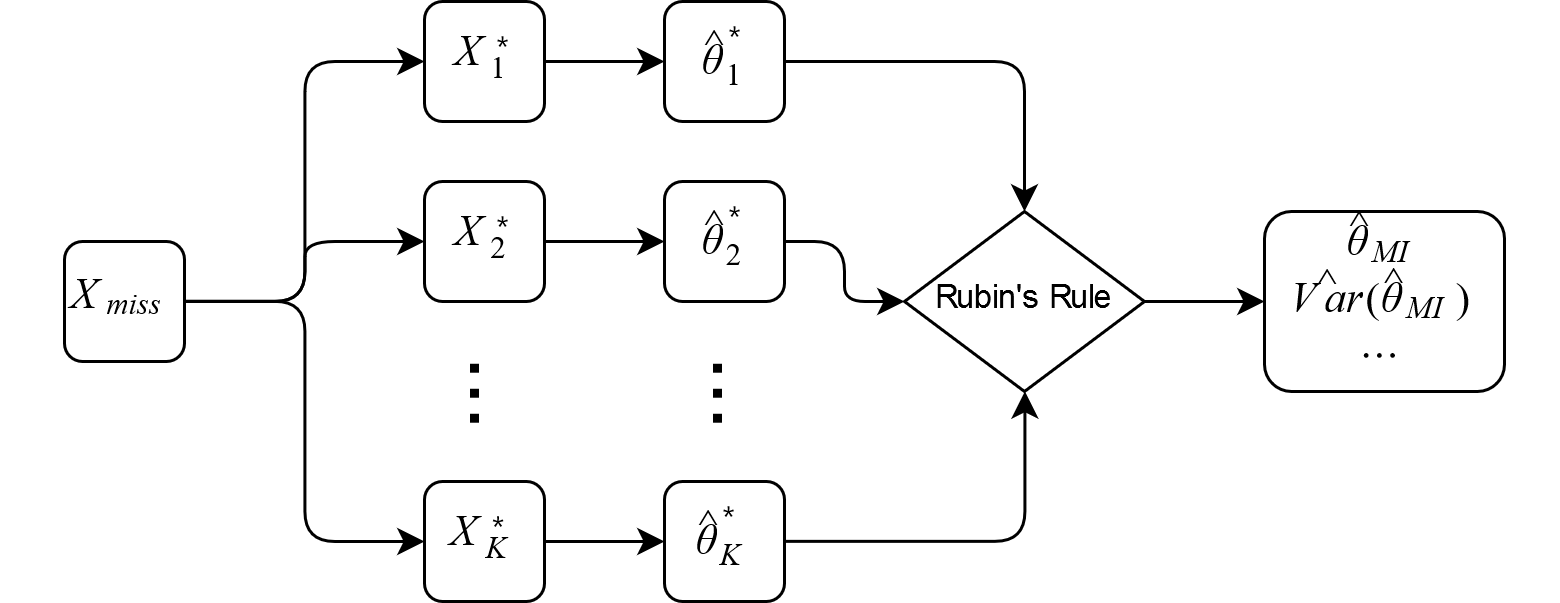
\includegraphics[width=0.9\paperwidth]{MI}
\end{frame}

\begin{frame}{Specification Overhead}
\begin{itemize}
\item Missingness pattern: MCAR, MAR, MNAR
\item Imputation model: linear regression, random forest, ...
\item Predictor vs response variables: leave-one-out, interactions, auxiliary, ...
\item Order of variable imputation: random, least/most missing first, ...
\item Initial imputations, number of iterations (convergence condition)
\item Number of multiply imputed datasets (cycles)
\end{itemize}
\end{frame}

\begin{frame}{Multiple Imputation by Chained Equations (MICE)}
$$X = \underbrace{\begin{pmatrix}
x_{11} 	& - 		& x_{13} \\
x_{21} 	& x_{22} 	& - \\
- 		& x_{32} 	& - \\
x_{41} 	& x_{42} 	& x_{43} \\
\end{pmatrix}}_\text{original design matrix}
\rightarrow
\underbrace{\begin{pmatrix}
x_{11} 		& \textcolor{red}{\bar{x}_{.2}} 	& x_{13} \\
x_{21} 		& x_{22} 		& \textcolor{red}{\bar{x}_{.3}} \\
\textcolor{red}{\bar{x}_{.1}} & x_{32} 	& \textcolor{red}{\bar{x}_{.3}} \\
x_{41} 		& x_{42} 	& x_{43} \\
\end{pmatrix}}_\text{initial imputation}
\rightarrow
\underbrace{\begin{pmatrix}
\textcolor{red}{\bar{x}_{.2}} 	& x_{13} \\
x_{22} 		& \textcolor{red}{\bar{x}_{.3}} \\
x_{42} 	& x_{43} \\
\end{pmatrix}}_\text{design matrix},
\underbrace{\begin{pmatrix}
x_{11} \\
x_{21} \\
x_{41} \\
\end{pmatrix}}_\text{response}$$

$$
\rightarrow
\begin{pmatrix}
x_{11} 		& \textcolor{red}{\bar{x}_{.2}} 	& x_{13} \\
x_{21} 		& x_{22} 		& \textcolor{red}{\bar{x}_{.3}} \\
\textcolor{blue}{\hat{x}_{31}} & x_{32} 	& \textcolor{red}{\bar{x}_{.3}} \\
x_{41} 		& x_{42} 	& x_{43} \\
\end{pmatrix}
\rightarrow
\begin{pmatrix}
x_{21} 		& \textcolor{red}{\bar{x}_{.3}} \\
\textcolor{blue}{\hat{x}_{31}} & \textcolor{red}{\bar{x}_{.3}} \\
x_{41} 		& x_{43} \\
\end{pmatrix},
\begin{pmatrix}
x_{22} \\
x_{32} \\
x_{42} \\
\end{pmatrix}
\rightarrow
\cdots
\underbrace{\begin{pmatrix}
x_{11} 		& \textcolor{blue}{\hat{x}_{12}} 	& x_{13} \\
x_{21} 		& x_{22} 		& \textcolor{blue}{\hat{x}_{23}} \\
\textcolor{blue}{\hat{x}_{31}} & x_{32} 	& \textcolor{blue}{\hat{x}_{33}} \\
x_{41} 		& x_{42} 	& x_{43} \\
\end{pmatrix}}_{X_i^{*}}
$$

\end{frame}

\begin{frame}{Deep Learning for Imputation}
Maybe explain this in detail as well? Depending on how complicated it is
\end{frame}


\section{Tools and libraries for dealing with missing data}

\begin{frame}{Visualization}
\end{frame}

\begin{frame}{Useful libraries}
\end{frame}

\section{Live Demo}

\appendix
\section{Backup}

\begin{frame}{Backup}
\scriptsize
test
\normalsize
\end{frame}

\end{document}
